\documentclass[12pt, letterpaper, twoside]{book}
\raggedbottom
\usepackage{graphicx}
\graphicspath{ {images/} }
\usepackage[utf8]{inputenc}
\usepackage{fullpage}
\usepackage[paperheight=11in,paperwidth=8.5in,margin=0in]{geometry}
\usepackage{amsmath}
\usepackage{listings}
\date{23nd May 2021}
\begin{document}
\begin{titlepage}
	\begin{center}
       \vspace*{5cm}
       \bfseries\Large
    	Assignment 2\\
    	Of\\
    	Modelling \& Simulation Lab (CS1052)\\
        \vskip1cm
        Masters of Technology in Computer Science And Engineering\\
        \vskip1cm
        submitted by\\
    	Arghya Bandyopadhyay\\
    	RollNo. 20CS4103\\
    	\vskip1cm
    	submitted to\\
    	Dr Nanda Dulal Jana\\
    	Assistant Professor\\
    	Dept. of CSE\\
    	\vskip1cm
    	
\includegraphics[width=4cm]{NITDGP}\\
    	National Institute of Technology, Durgapur\\
    \end{center}
\end{titlepage}
\begin{center}
\textbf{\\Problem 1}
\end{center}
\begin{flushleft}
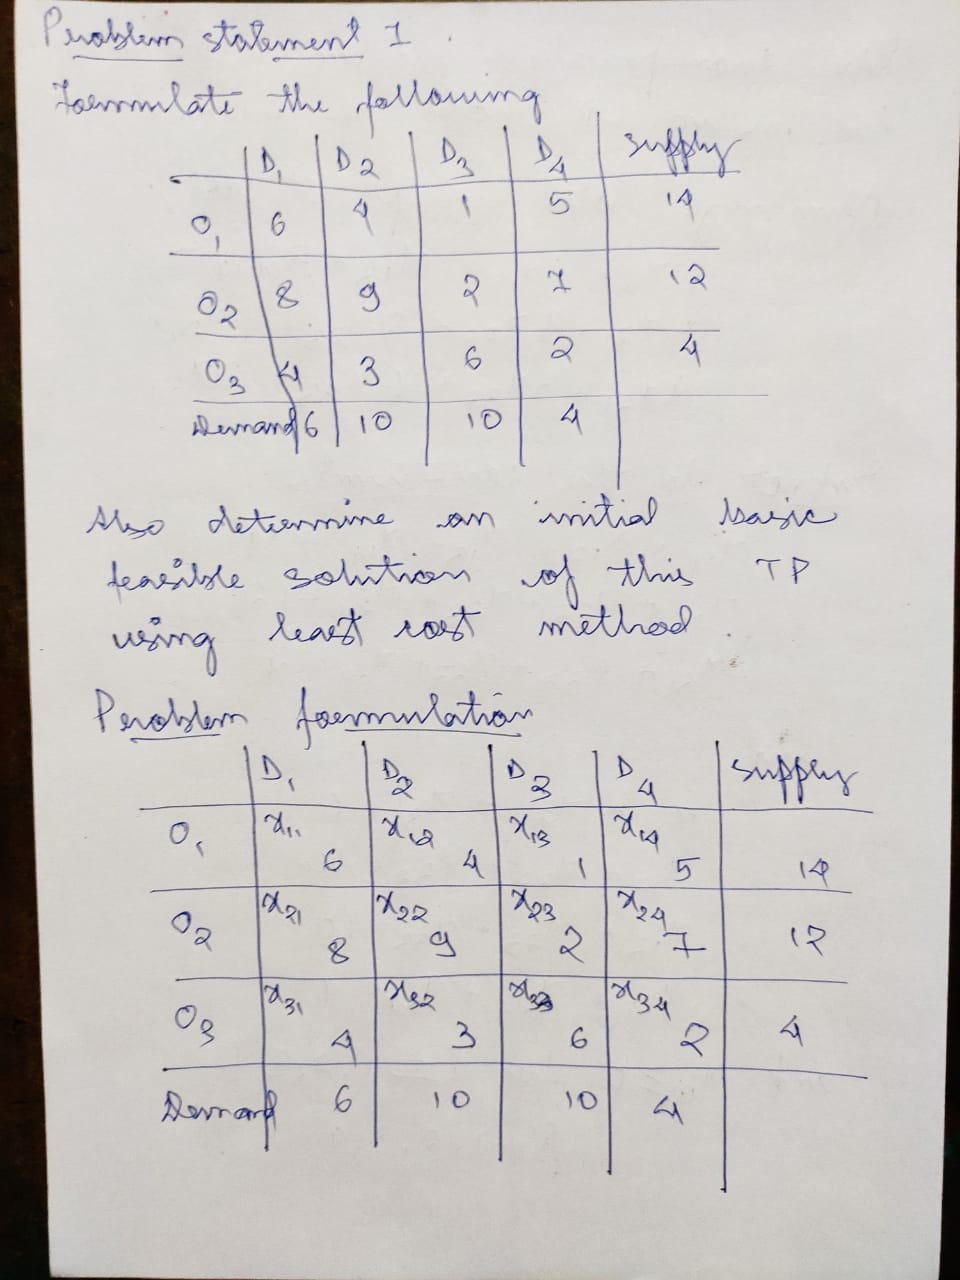
\includegraphics[width=\paperwidth, height=10in]{Page1}
\end{flushleft}
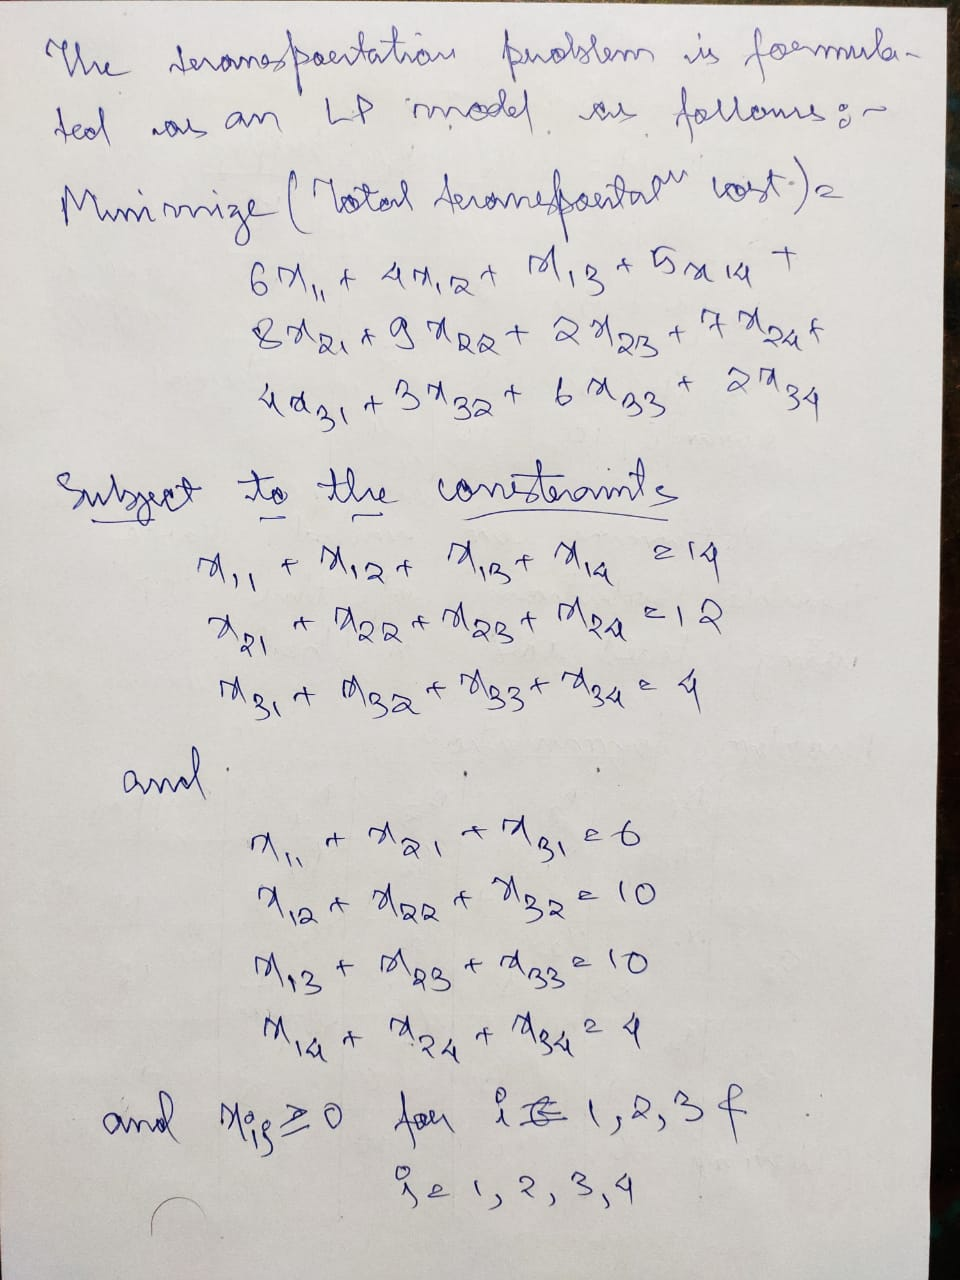
\includegraphics[width=\paperwidth, height=\paperheight]{Page2}
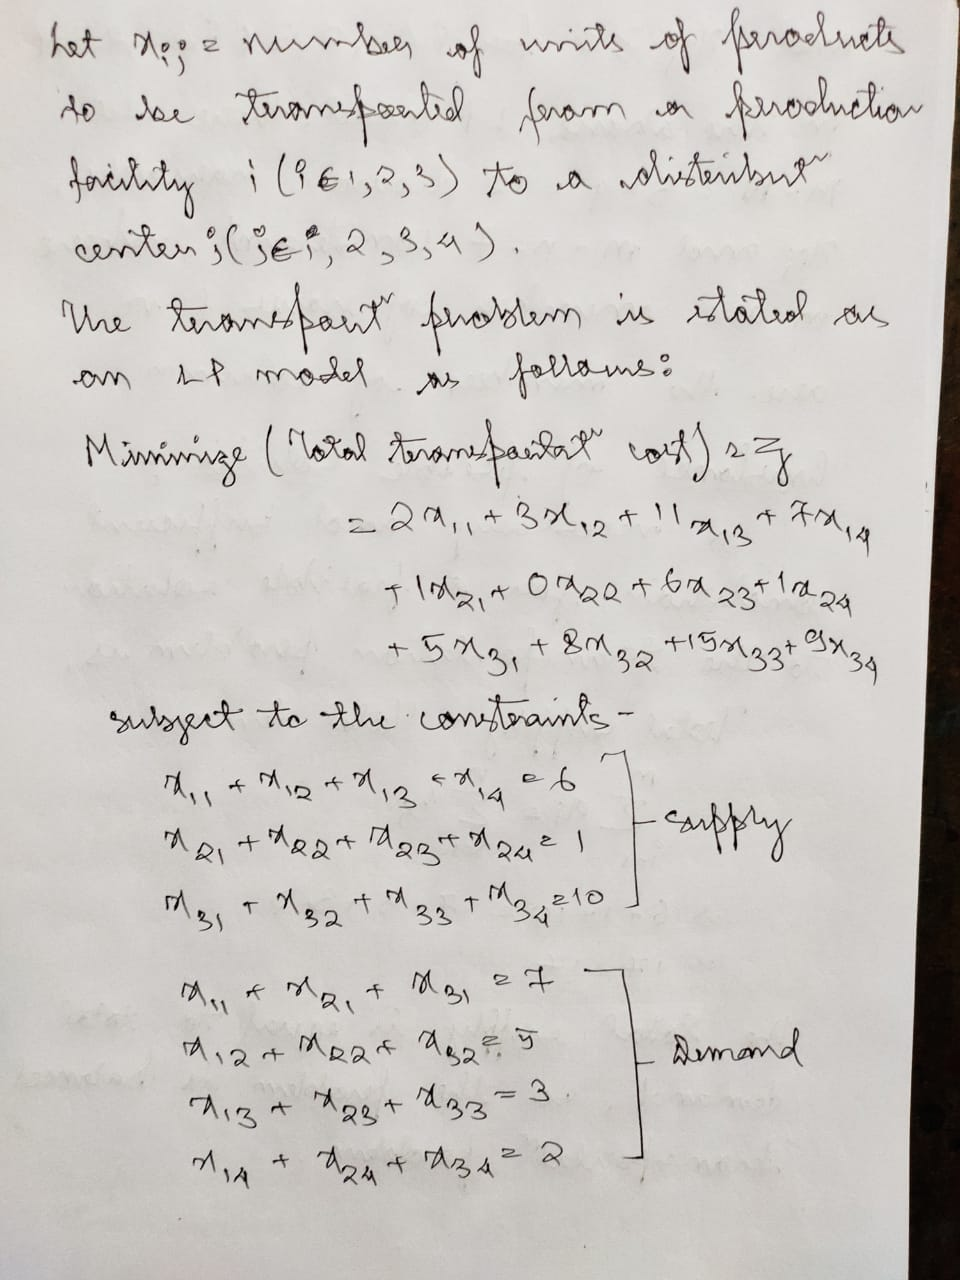
\includegraphics[width=\paperwidth, height=\paperheight]{Page3}
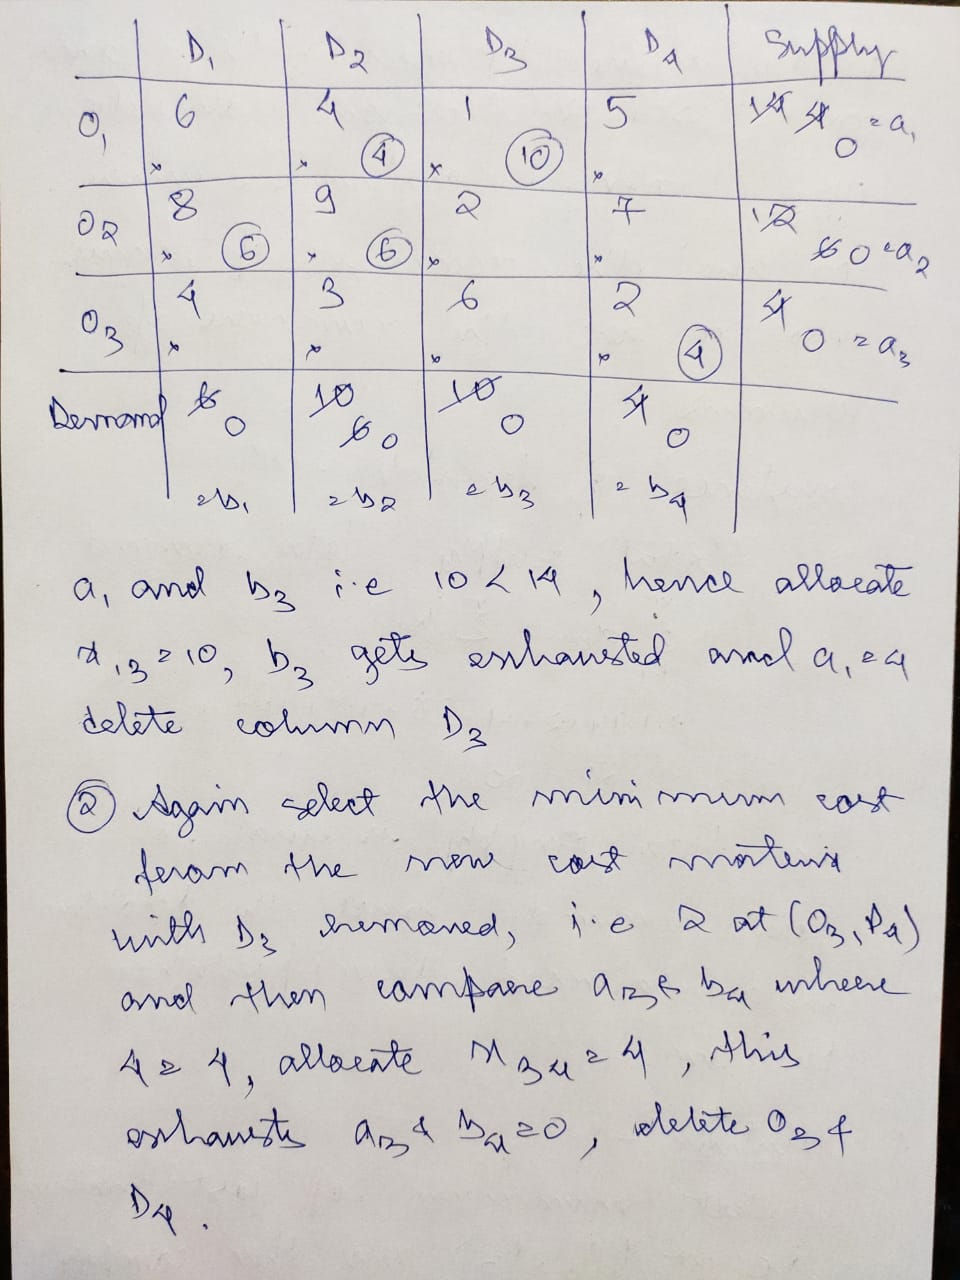
\includegraphics[width=\paperwidth, height=\paperheight]{Page4}
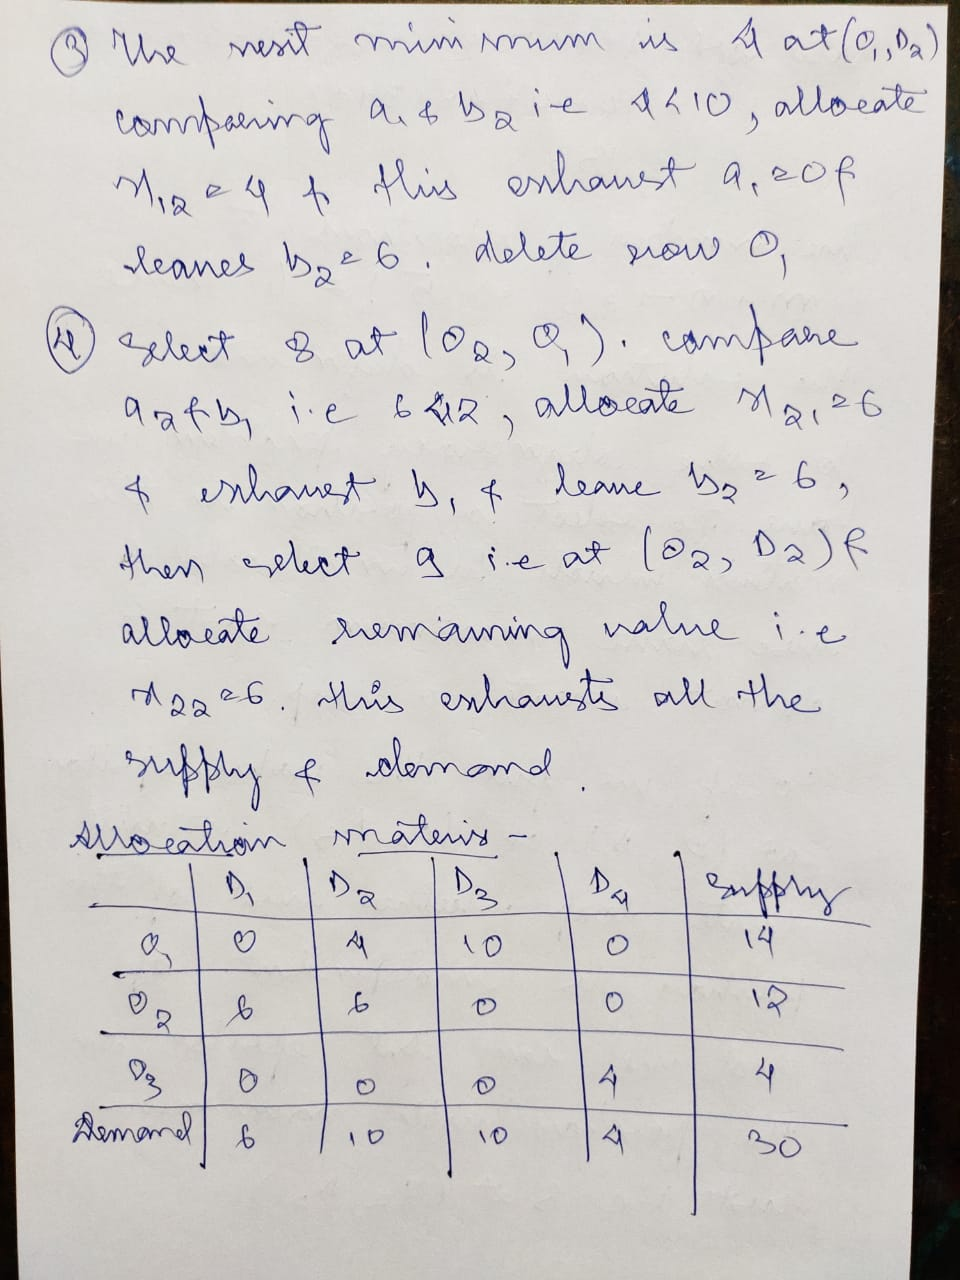
\includegraphics[width=\paperwidth, height=\paperheight]{Page5}
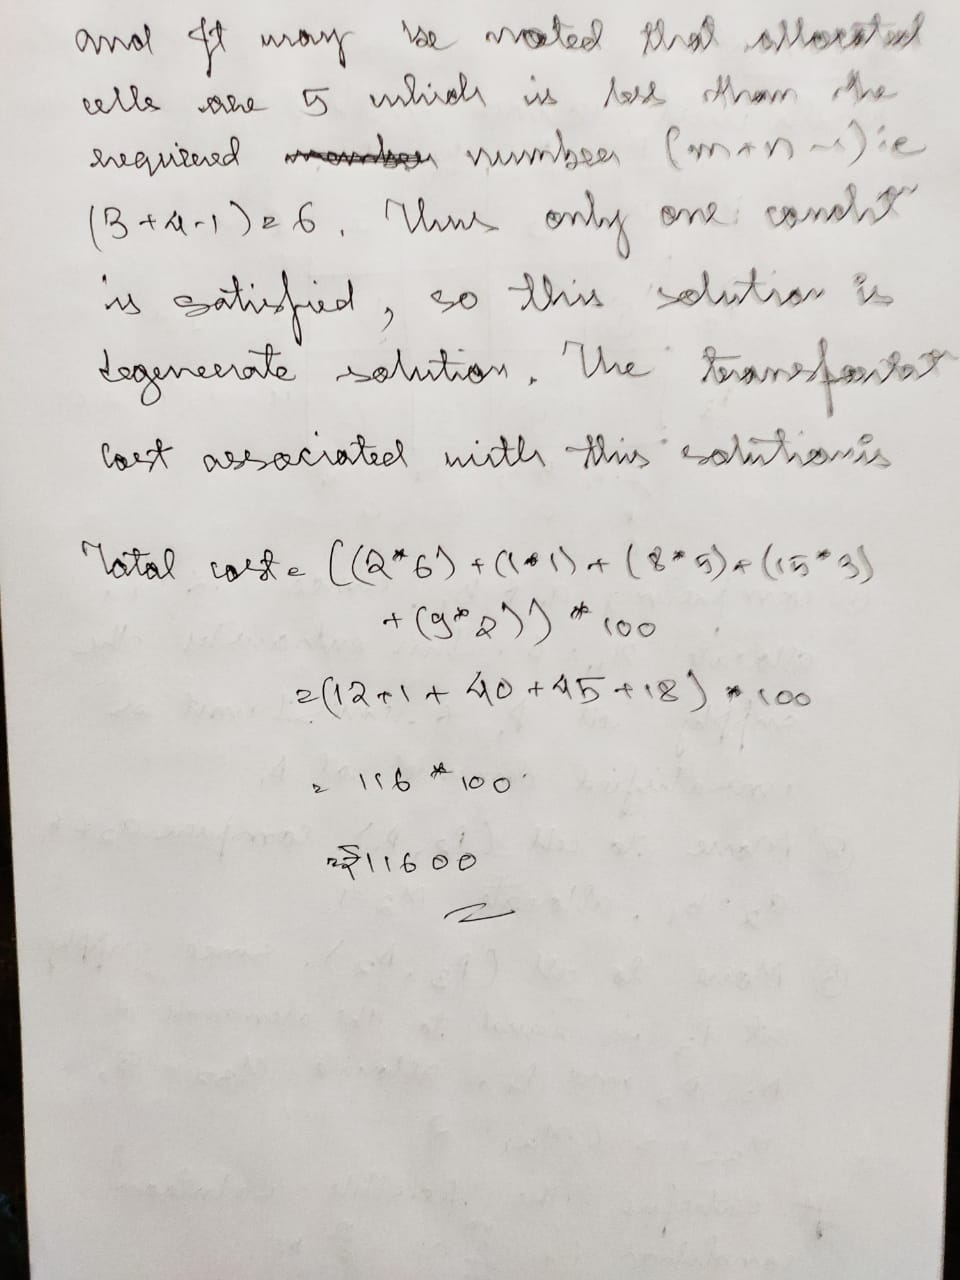
\includegraphics[width=\paperwidth, height=\paperheight]{Page6}
\begin{lstlisting}

	Python Code:
	
	import numpy as np
	
	if __name__ == '__main__':
		total_cost = 0
		no_alloc = 0
		
		# initiatizes the cost matrix
		cm = np.array([
			[9, 12, 9, 6, 9, 10, 5], 
			[7, 3, 7, 7, 5, 5, 6], 
			[6, 5, 9, 11, 3, 11, 2], 
			[6, 8, 11, 2, 2, 10, 9],
			[4, 4, 6, 2, 4, 2, 0]])
		print("Cost Matrix")
		
		# prints the cost matrix
		print(cm)
		
		# calculates the no of rows and columns
		r, c = cm.shape
		print("Rows, Columns: (", r - 1, ",", c - 1, ")")
		
		# slices the cost matrix to get the sum of the demand 
		# and supply vectors
		total_demand = np.sum(cm[r - 1, :])
		total_supply = np.sum(cm[:, c - 1])
		if total_demand == total_supply:
			print("Balanced Transportation Problem.")
		else:
			print("Unbalanced Transportation Problem")
		i = 0
		j = 0
		
		# This loop does allocation to the cells according to
		# the requirement and possible supply
		while (i < r - 1) and (j < c - 1):
			x = min(cm[r - 1, j], cm[i, c - 1])
			cm[r - 1, j] = cm[r - 1, j] - x
			cm[i, c - 1] = cm[i, c - 1] - x
			total_cost = total_cost + x * cm[i, j]
			no_alloc = no_alloc + 1
			if cm[r - 1, j] < cm[i, c - 1]:
				j = j + 1
			elif cm[r - 1, j] > cm[i, c - 1]:
				i = i + 1
			else:
				i = i + 1
				j = j + 1
			print("Total Cost: ", total_cost)
			print("No of Allocation: ", no_alloc)
			
			
			
			
			# checks for the condition m+n-1 = no of allocated cells
			if ((r - 1) + (c - 1) - 1) == no_alloc and 
					total_demand == total_supply:
				print("Non Degenerate & Feasible Solution")
			else:
				print("Degenerate Solution")
	
	Output:

\end{lstlisting}

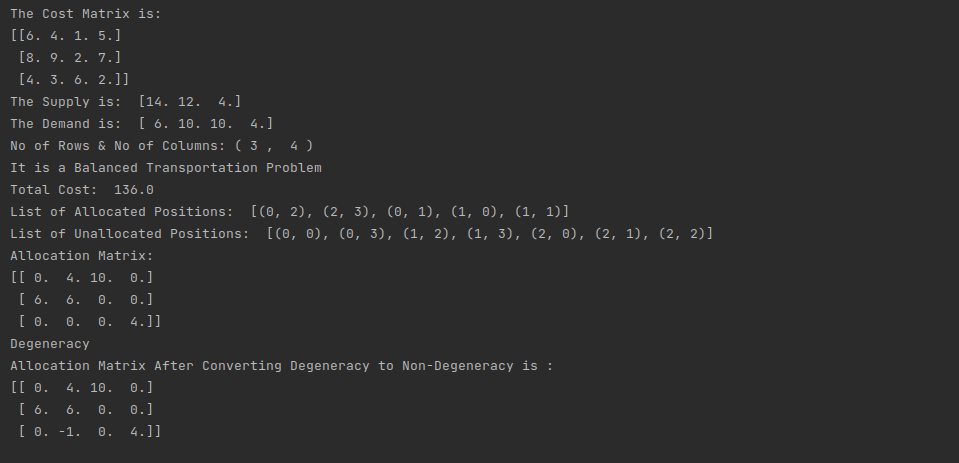
\includegraphics[height=600pt,width=550pt]{Output1}

\begin{center}
\textbf{\\Problem 2}
\end{center}

\begin{flushleft}
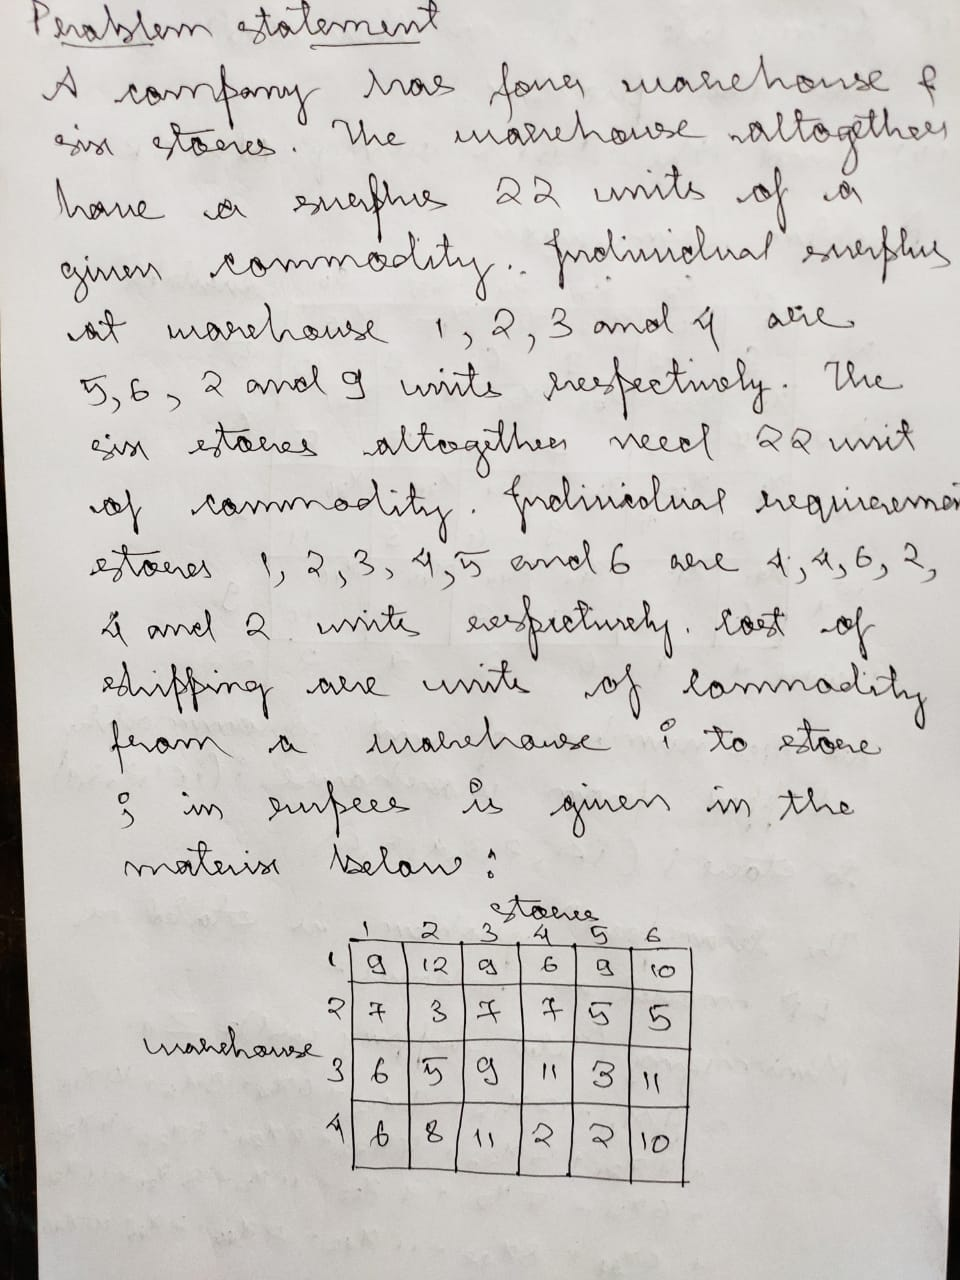
\includegraphics[width=\paperwidth, height=10in]{Page7}
\end{flushleft}
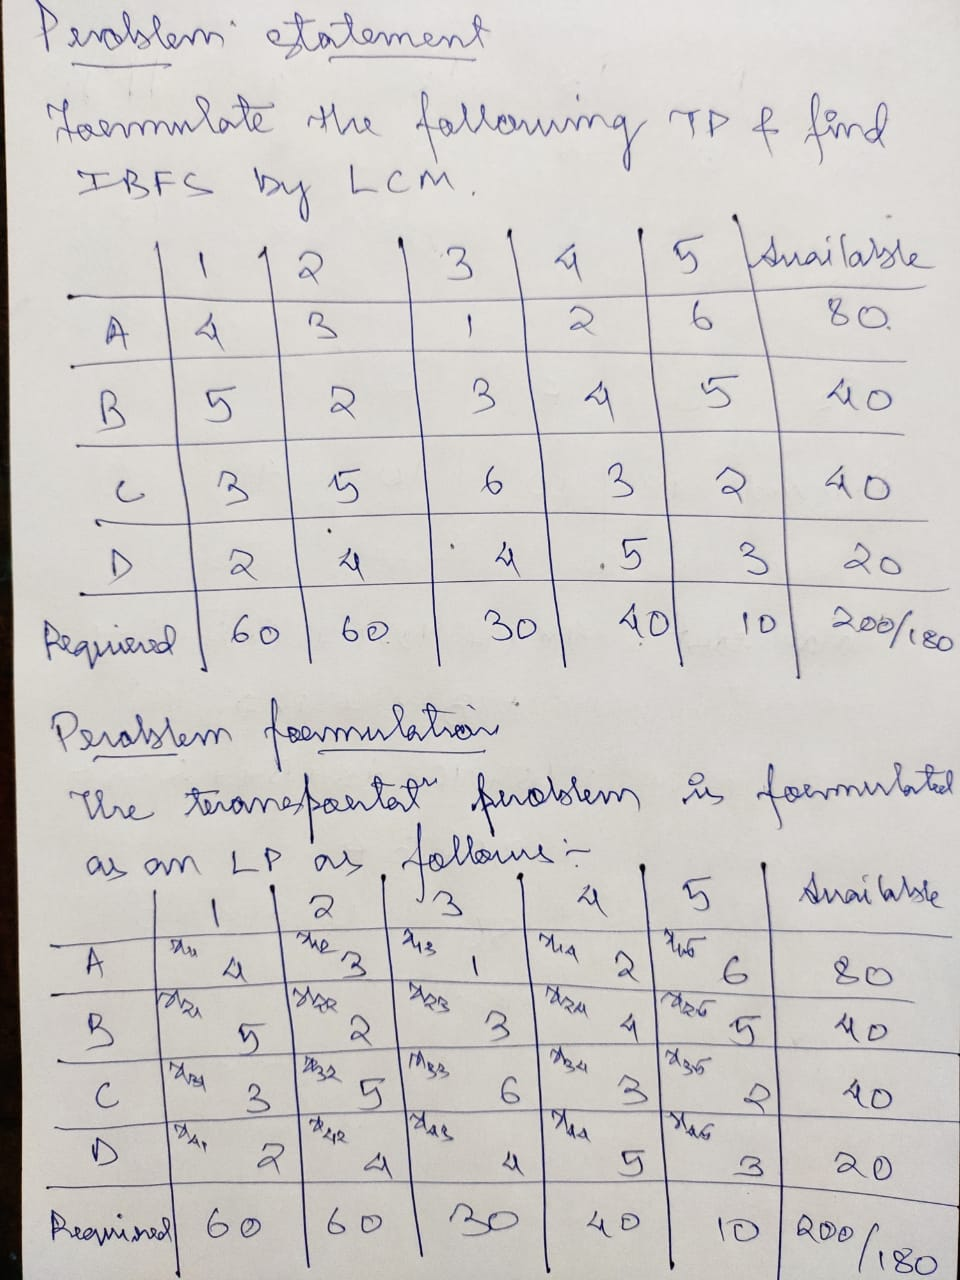
\includegraphics[width=\paperwidth, height=\paperheight]{Page8}
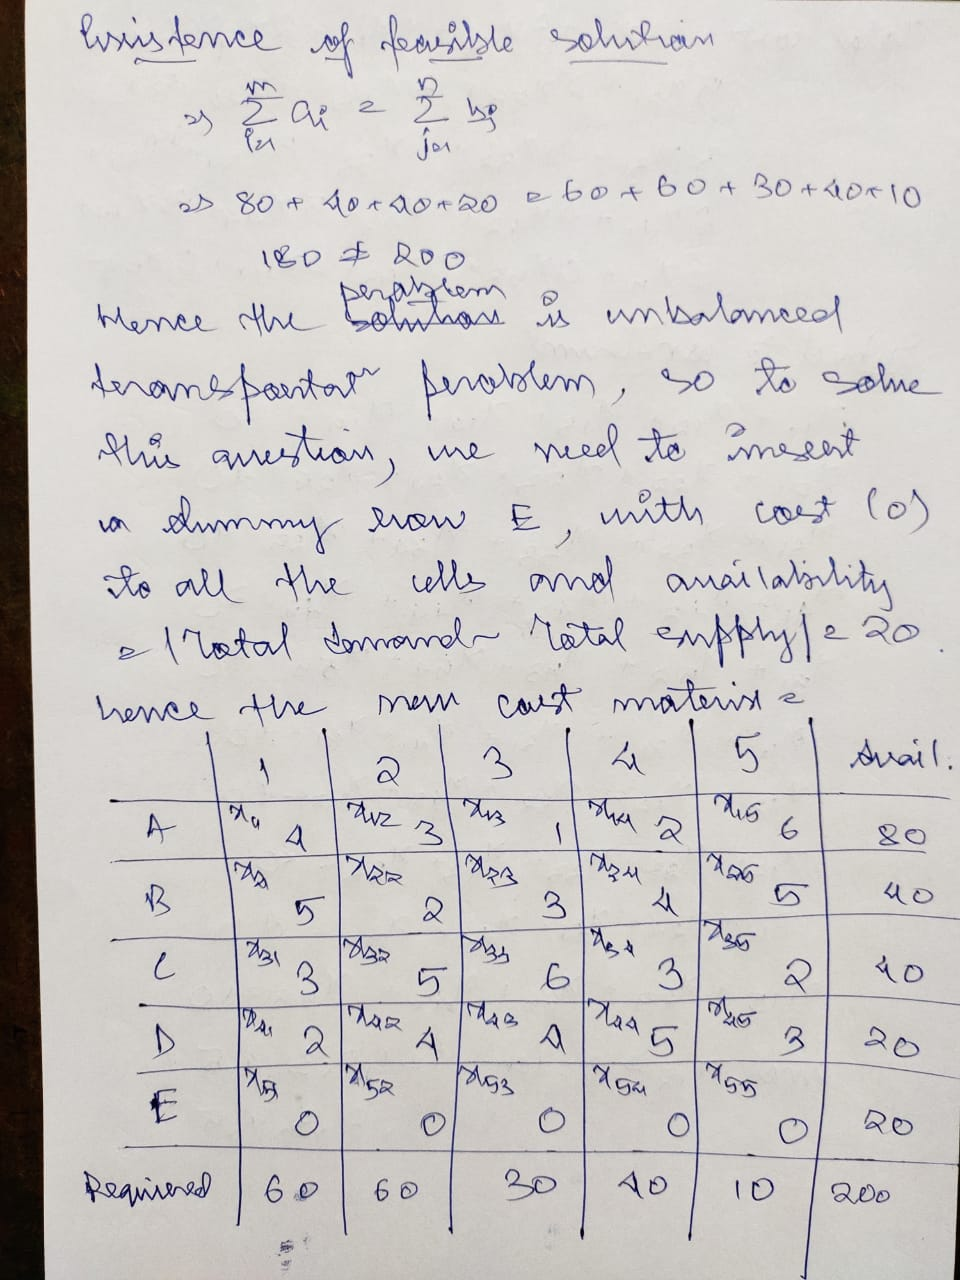
\includegraphics[width=\paperwidth, height=\paperheight]{Page9}
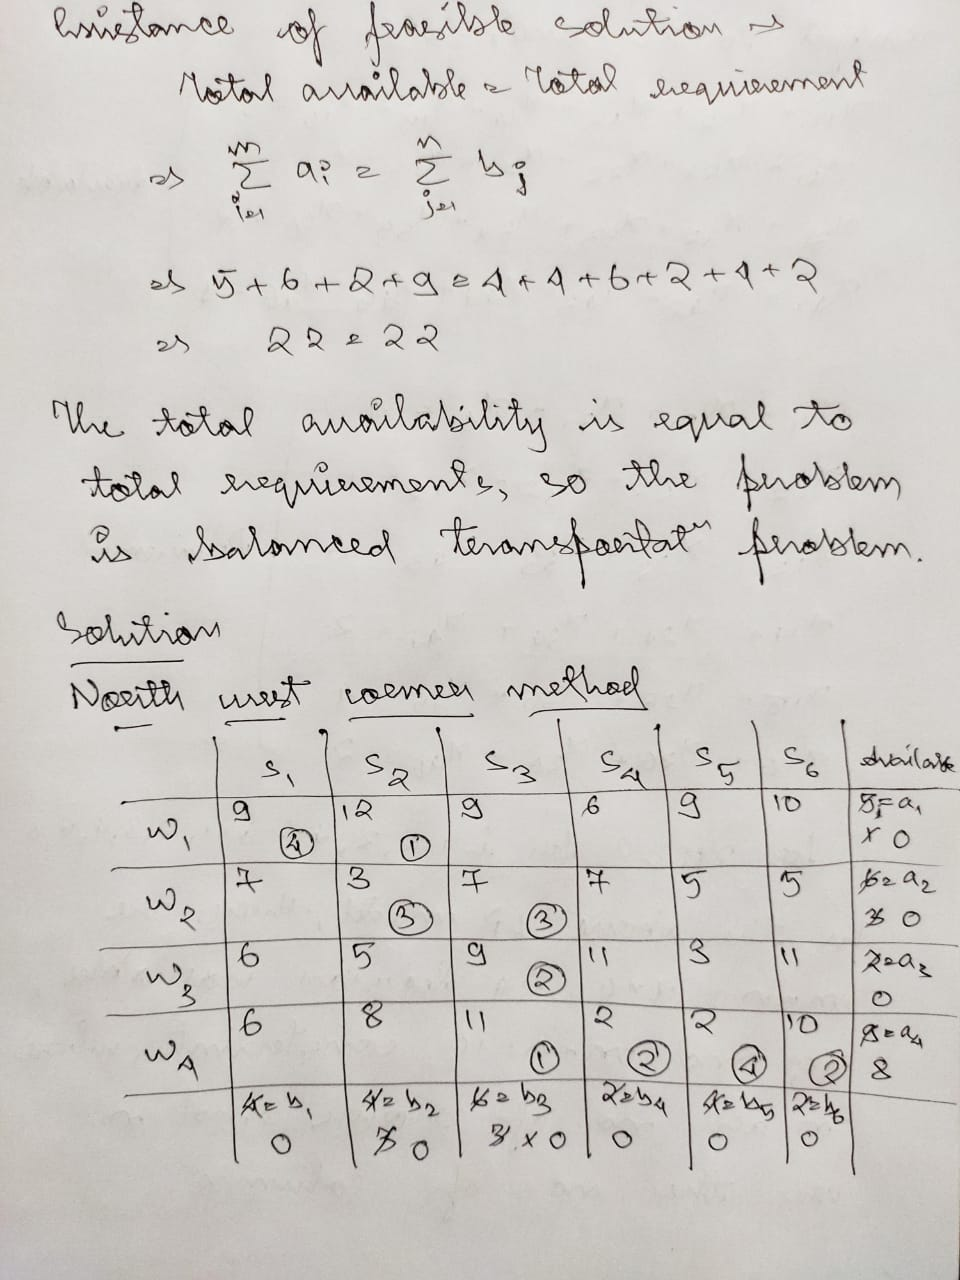
\includegraphics[width=\paperwidth, height=\paperheight]{Page10}
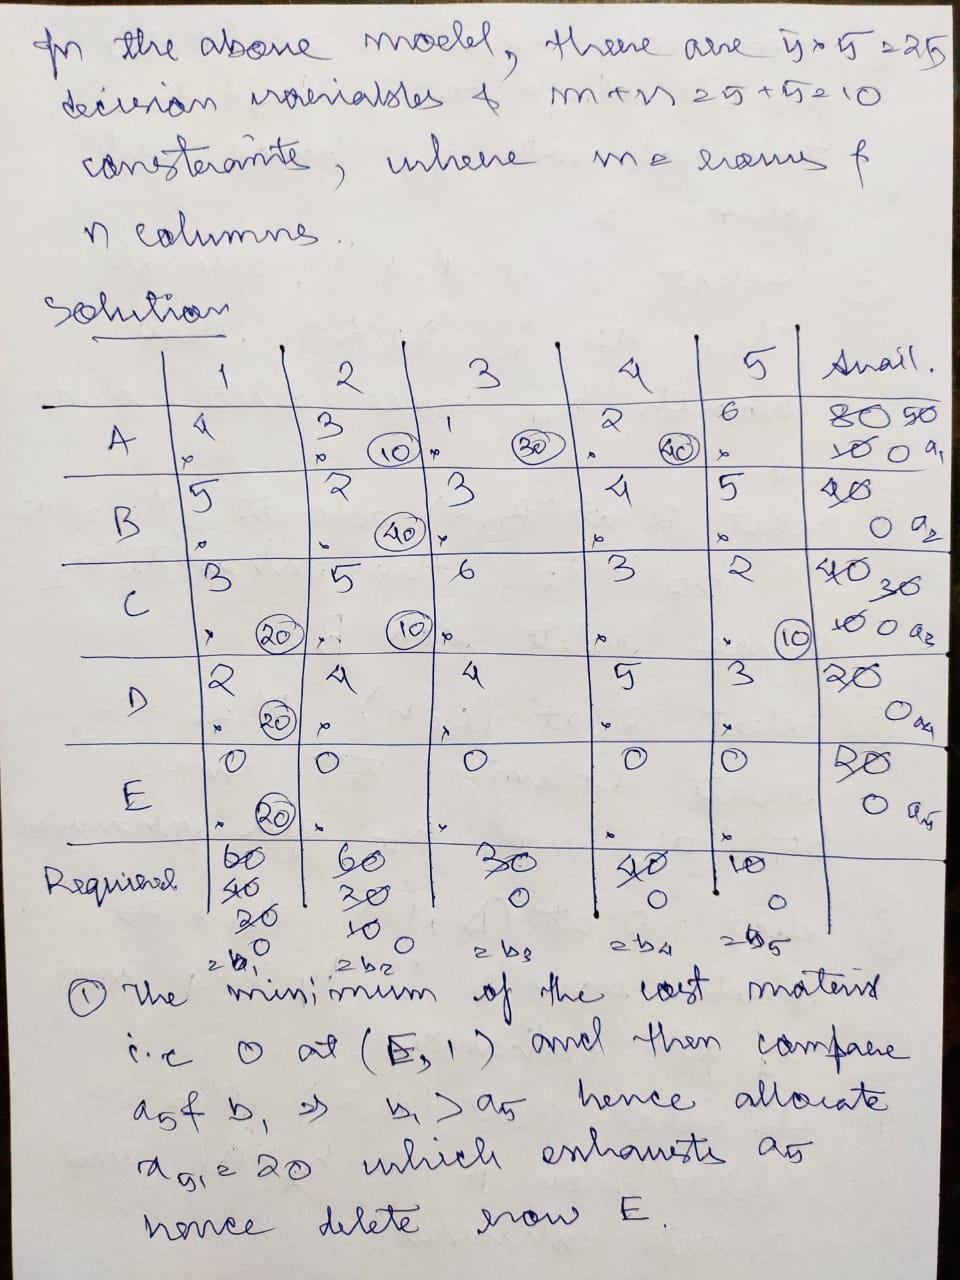
\includegraphics[width=\paperwidth, height=\paperheight]{Page11}
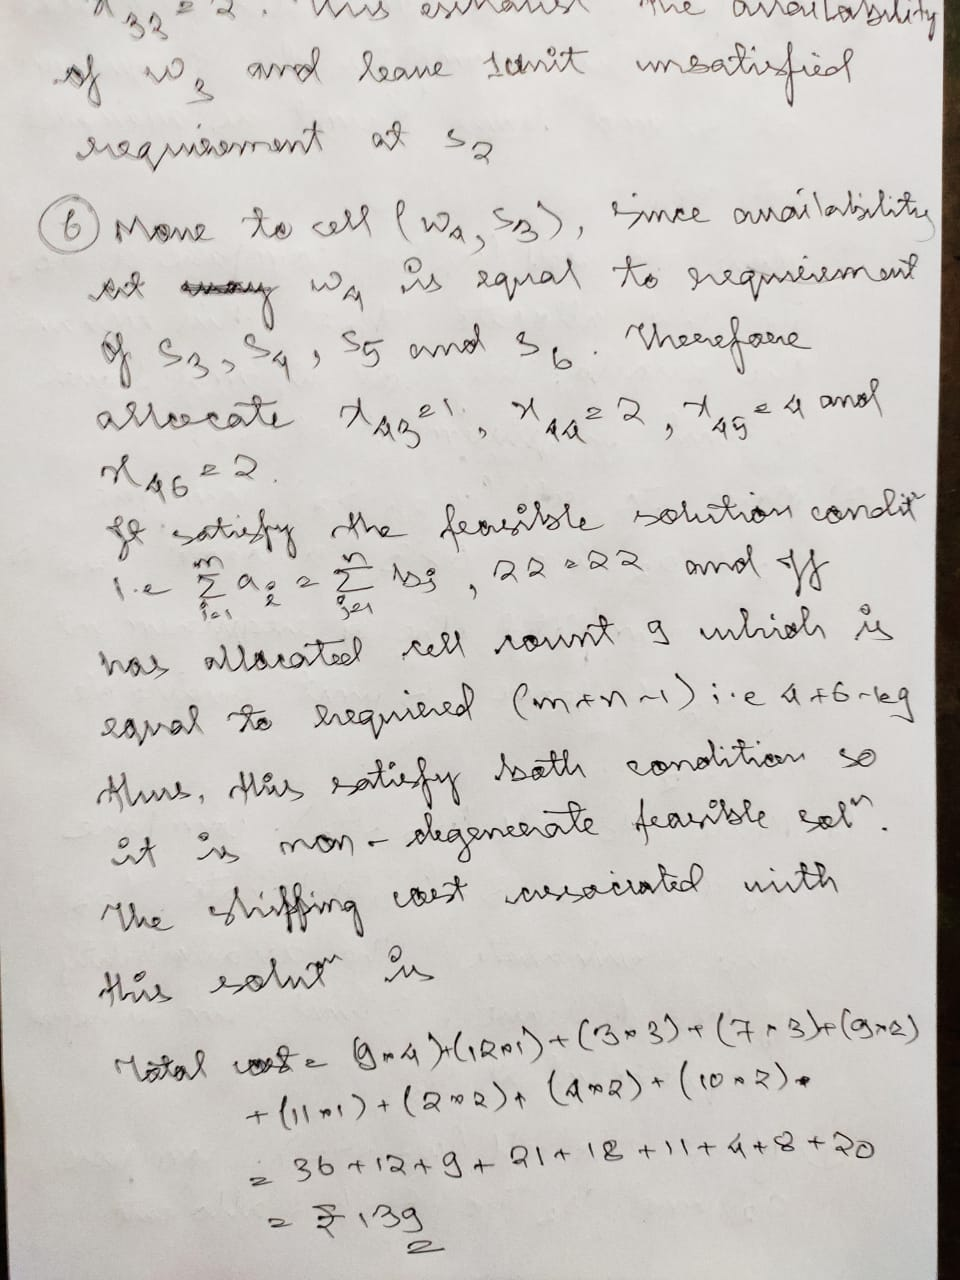
\includegraphics[width=\paperwidth, height=\paperheight]{Page12}
\begin{lstlisting}

	Python Code:
	
	import numpy as np
	
	if __name__ == '__main__':
		total_cost = 0
		no_alloc = 0
		
		# initiatizes the cost matrix
		cm = np.array([
		[2, 3, 11, 7, 6], 
		[1, 0, 6, 1, 1], 
		[5, 8, 15, 9, 10], 
		[7, 5, 3, 2, 0]])
		print("Cost Matrix")
		
		# prints the cost matrix
		print(cm)
		
		# calculates the no of rows and columns
		r, c = cm.shape
		print("Rows, Columns: (", r - 1, ",", c - 1, ")")
		
		# slices the cost matrix to get the sum of the demand 
		# and supply vectors
		total_demand = np.sum(cm[r - 1, :])
		total_supply = np.sum(cm[:, c - 1])
		if total_demand == total_supply:
			print("Balanced Transportation Problem.")
		else:
			print("Unbalanced Transportation Problem")
		i = 0
		j = 0
		
		# This loop does allocation to the cells according to
		# the requirement and possible supply
		while (i < r - 1) and (j < c - 1):
			x = min(cm[r - 1, j], cm[i, c - 1])
			cm[r - 1, j] = cm[r - 1, j] - x
			cm[i, c - 1] = cm[i, c - 1] - x
			total_cost = total_cost + x * cm[i, j]
			no_alloc = no_alloc + 1
			if cm[r - 1, j] < cm[i, c - 1]:
				j = j + 1
			elif cm[r - 1, j] > cm[i, c - 1]:
				i = i + 1
			else:
				i = i + 1
				j = j + 1
			print("Total Cost: ", total_cost * 100)
			print("No of Allocation: ", no_alloc)
			
			
			
			
			# checks for the condition m+n-1 = no of allocated cells
			if ((r - 1) + (c - 1) - 1) == no_alloc and 
					total_demand == total_supply:
				print("Non Degenerate & Feasible Solution")
			else:
				print("Degenerate Solution")
	
	Output:

\end{lstlisting}

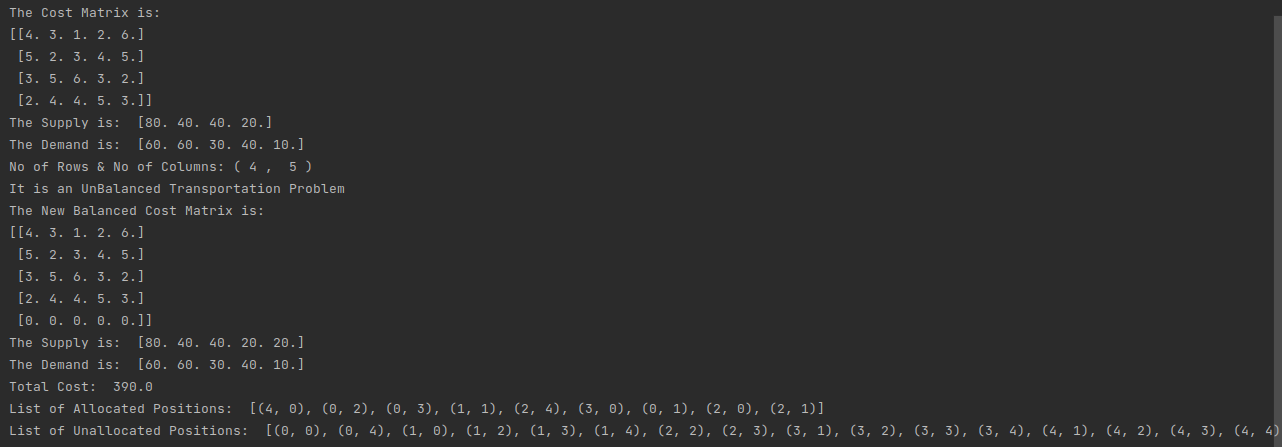
\includegraphics[height=400pt,width=550pt]{Output2}


\includegraphics[height=200pt,width=550pt]{Output3}
\end{document}
